
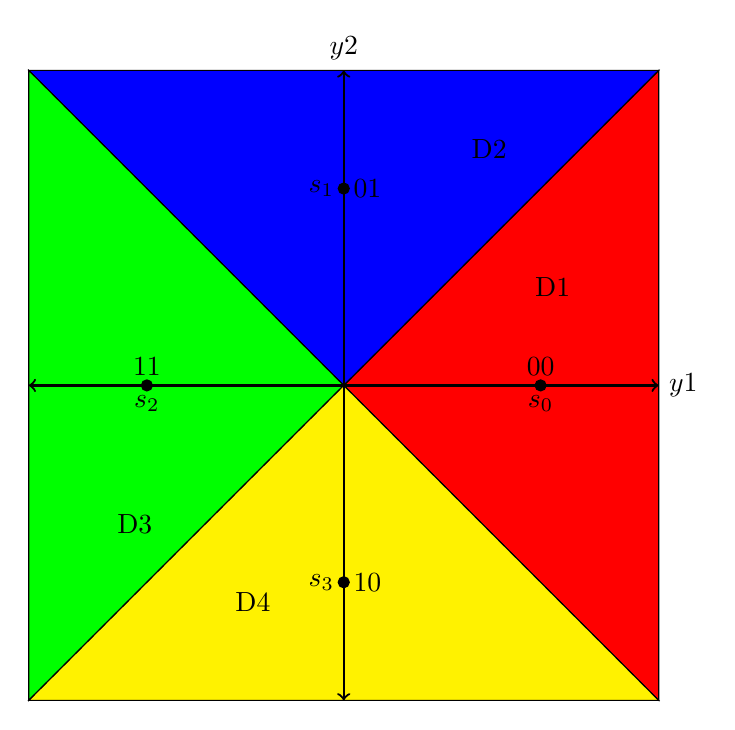
\begin{tikzpicture}


\draw[fill=red]  (0,0) -- (4,4) -- (4,-4)  -- cycle;

\draw[fill=blue]  (0,0) -- (4,4) -- (-4,4)  -- cycle;
\draw[fill=green]  (0,0) -- (-4,4) -- (-4,-4)  -- cycle;
\draw[fill=yellow]  (0,0) -- (-4,-4) -- (4,-4)  -- cycle;



\draw[<->,thick] (-4,0)--(4,0) node[right]{$y1$};
\draw[<->,thick] (0,-4)--(0,4) node[above]{$y2$};
\draw [dashed]   (-4,-4)--(4,4);
\draw [dashed]   (-4,4)--(4,-4);

\filldraw[black] (2.5,0) circle (2pt) node[below] {$s_0$} node[above] {00};
\filldraw[black] (0,2.5) circle (2pt) node[left] {$s_1$} node[right] {01};
\filldraw[black] (-2.5,0) circle (2pt) node[below] {$s_2$} node[above] {11};
\filldraw[black] (0,-2.5) circle (2pt) node[left] {$s_3$} node [right] {10} ;


\foreach \coordinate/\label/\pos in {{(3,1)/D1/above left},{(1.5,3)/D2/right},{(-3,-2)/D3/above right},{(-1.5,-3)/D4/above right}} \node[\pos] at \coordinate {\label};

\end{tikzpicture}
